\documentclass[12pt,a4paper]{article}
\usepackage[latin1]{inputenc}
\usepackage{amsmath}
\usepackage{amsfonts}
\usepackage{amssymb}
\usepackage{graphicx}
\usepackage{subfig, placeins}
\usepackage[left=1.00in, right=1.00in, top=1.00in, bottom=1.00in]{geometry}
\begin{document}
\noindent Noah Dukler

Data for this project were derived from 79 chinese and 107 Yoruban individuals for a total study size of 186 people. The gender breakdown was 92 females and 94 males however only SNP data for chromosome 22 was included for this study so sex specific effects are highly unlikely. SNP data was filtered to remove alleles with MAF$<0.05$ resulting in the removal of 562 variants. All individuals were completely genotyped so none were removed. Re-clustering all study individuals based on genotype cleanly recapitulated the ethnic labeling in the HapMap files along the 1st PC with no obvious outliers so no individuals appear to be mislabeled (fig. \ref{fig:mds}). Individuals were not separated by sex along any of the other PCs as expected since the sex chromosomes were not included.   

\begin{figure}[h]
\centering
\includegraphics[width=0.9\linewidth]{../test/cluster_info/mds}
\caption[MDS Plot]{MDS Plot of filtered genotypes. Individuals cleanly separate by ethnicity along PC1 but fail to separate by gender.}
\label{fig:mds}
\end{figure}

The phenotypes of interest were the expression levels of three genes GGT5, MRPL40, and TTC38. The distributions of expression levels were then checked for normality. 

\begin{figure}[h]
\centering
\includegraphics[width=0.9\linewidth, height=7cm]{../test/processed_files/pheno_dist}
\caption[Pheno_dist]{Distribution of expression levels for GGT5, MRPL40, and TTC38 across study population. Data were tested for normality with the Shapiro-Wilk test. Expression data for MPRL and GGT5 were normally distributed with $p>0.05$. Expression levels for TTC38 were non normally distributed with $p<<0.05$.}
\label{fig:pheno_dist}
\end{figure}

The data for TTC38 were strongly non-normally distributed, violating the assumption of the regression model risking an increased false positive rate so I performed quantile renormalization on all three phenotypes for consistent data treatment \cite{goh_effects_2009}. Using PLINK I fit the data to a naive association model of the form:

$$
	Norm.~Gene~Expression = Genotype + \epsilon
$$

Genotypes are recoded as $aa=0$, $Aa=1$, and $AA=2$, giving a unique encoding to all allelic combinations. However the p-values resulting from this analysis were left-highly skewed indicating that there would be a high false positive rate resulting from this analysis (fig. \ref{norm_assoc}). 

\begin{figure}
\subfloat[GGT5 \label{fig3:test1}]
  {\includegraphics[width=.3\linewidth]{../test/norm_basic.plink/plots/pplot_GGT5.pdf}}\hfill
\subfloat[MRPL40 \label{fig3:test2}]
  {\includegraphics[width=.3\linewidth]{../test/norm_basic.plink/plots/pplot_MRPL40.pdf}}\hfill
\subfloat[TTC38\label{fig3:test3}]
  {\includegraphics[width=.3\linewidth]{../test/norm_basic.plink/plots/pplot_TTC38.pdf}}
\caption{Histogram and qqplot of p-values derived from fitting basic association model to rank normalized expression data for three genes.}
\label{norm_assoc}
\end{figure}   

This inflation in the frequency of low p-values often results from unmodeled substructure in the population. From our PCA analysis we already know that the study population clusters into two distinct subpopulations based upon ethnicity. Therefore we revise our previous model to include a covariate to model ethnic background as follows: 

$$
	Norm.~Gene~Expression = Genotype + Ethnicity +\epsilon
$$

Ethnicity was recoded by representing CHB individuals as 1 and YRIs as 2. The p-values resulting from fitting this second model were almost uniformly distributed showing that the majority of loci failed to reject the null-hypothesis as expected (aka. were non-causal). Given that the effects of population substructure appear to have been accounted for I proceeded to search for causal loci for the three traits of interest. 

\begin{figure}
\subfloat[GGT5 \label{fig4:test1}]
  {\includegraphics[width=.3\linewidth]{../test/pop_covar.plink/plots/pplot_GGT5.pdf}}\hfill
\subfloat[MRPL40 \label{fig4:test2}]
  {\includegraphics[width=.3\linewidth]{../test/pop_covar.plink/plots/pplot_MRPL40.pdf}}\hfill
\subfloat[TTC38\label{fig4:test3}]
  {\includegraphics[width=.3\linewidth]{../test/pop_covar.plink/plots/pplot_TTC38.pdf}}
\caption{Histogram and qqplot of p-values derived from fitting an association model that includes ethnicity to rank normalized expression data for three genes.}
\label{covar_pp}
\end{figure}

\begin{figure}
\caption{Manhattan plots of p-values derived from fitting an association model that includes ethnicity to rank normalized expression data for three genes.}
\label{fig:merged_mhplot}
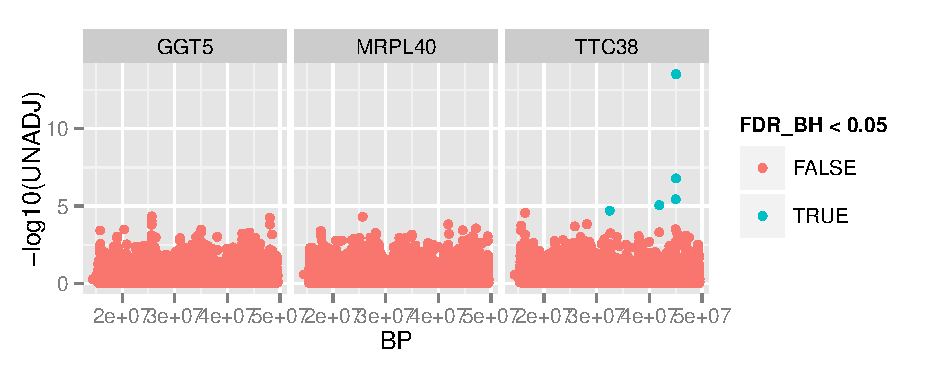
\includegraphics[width=1\linewidth]{./merged_mhplot}
\end{figure}

Of the three genes only one, TTC38 appeared to have any causal eQTLs on chromosome 22 between 14430353 and 49565872bp. Five eQTLs were identified of which 

\begin{table}[h]
\centering
\begin{tabular}{llrr}
  \hline
GENE & SNP & BP & FDR\_BH \\ 
  \hline
TTC38 & rs5999089 & 32484444 & 0.05 \\ 
  TTC38 & rs6008538 & 45064627 & 0.00 \\ 
  TTC38 & rs6008598 & 45082907 & 0.00 \\ 
  TTC38 & rs6971 & 41888870 & 0.02 \\ 
  TTC38 & rs9626816 & 45020262 & 0.01 \\ 
   \hline
\end{tabular}
\caption[eQTL]{Causal eQTLs identified by model that included ethnic covariate.}
\end{table}


\FloatBarrier
\bibliography{GWAS}
\bibliographystyle{plain}

\end{document}